\documentclass[11pt]{article}

\usepackage{geometry, fancyhdr, tikz, float, courier, chngcntr}
\usetikzlibrary{snakes}

\title{The Ekans Webserver \\ {\small\textbf{Software Design Specification}}}
\author {Samuel C. Payson}
\date{{\footnotesize \emph{last modified\\}}\today}

\counterwithin{figure}{section}

\begin{document}
\maketitle
\thispagestyle{empty}
\pagebreak
\pagestyle{fancy}
\setcounter{page}{1}
\pagenumbering{roman}
\tableofcontents
\pagebreak
\setcounter{page}{1}
\pagenumbering{arabic}
\section{Introduction}
Ekans is a lightweight webserver designed to quickly serve static content, while allowing for dynamic content powered by a Python backend. The initial section of this document provides a concise high-level overview of the server's design, followed by more detailed sections explaining the implementation of each of the server's main modules.
\subsection{The Ekans Design Mentality}
Ekans' design follows the mindset of the procedural paradigm. Data and procedures are \emph{distinct} (unlike in object oriented design) and the program is divided into large cohesive modules, rather than small compartmentalized objects.



\subsection{Understanding Figures}
The flowcharts and figures throughout this document attempt to follow the same general guidelines for design in order to be as useful as possible. The following are a set of informal rules for the interpretation of figures. Every figure in this document is accompanied by some form of text description, however. This description should always take priority over the following guidelines.
\subsubsection{Arrows}
In a given flowchart, there may be three kinds of arrows, each with the following meanings.
\begin{enumerate}
  \item[\tikz{\draw[fill=white,draw=white](0,-0.1) rectangle (0.8,0.1);\draw[thick,->,raise snake=0.2](0,0)--(0.8,0);}] The solid arrow indicates the movement of data. For example, the code
    \begin{center}
      \begin{tabular}{l}
        \texttt{\textbf{somefunction}(\&some\_data);} \\
        \texttt{\textbf{otherfunction}(\&some\_data);}
      \end{tabular}
    \end{center}
    might be represented as
    \begin{center}
      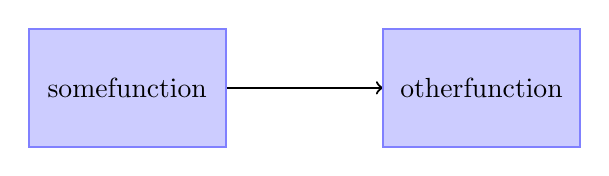
\begin{tikzpicture}
        \draw[thick,->] (-1.0, 0) -- (1.0, 0);
        \draw[fill=blue!20,draw=blue!50,thick] (1.0,-0.75) rectangle (3.5,0.75);
        \draw[fill=blue!20,draw=blue!50,thick] (-3.5,-0.75) rectangle (-1.0,0.75);
        \path (-2.25, 0) node {somefunction};
        \path ( 2.25, 0) node {otherfunction};
      \end{tikzpicture}
    \end{center}
    The diagram indicates that data is processed by \textbf{somefunction}, then passed on to \textbf{otherfunction}.
    \pagebreak
  \item[\tikz{\draw[fill=white,draw=white](0,-0.1) rectangle (0.8,0.1);\draw[thin, densely dashed,->,raise snake=0.2](0,0)--(0.8,0);}] The dashed arrow indicates a link of some sort. It could be a pointer, a TCP connection, or something more abstract. For example, a linked list might appear as
    \begin{center}
      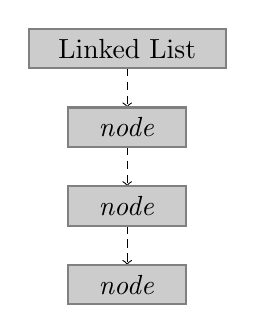
\begin{tikzpicture}[
          link/.style={densely dashed,->,thin},
          node/.style={fill=black!20,draw=black!50,thick},
        ]

        \draw[link] (0, 2.5) -- (0, 2);
        \draw[link] (0, 1.5) -- (0, 1);
        \draw[link] (0, 0.5) -- (0, 0);

        \draw[node] (-1.25, 3) rectangle (1.25, 2.5);
        \draw[node] (-0.75, 2) rectangle (0.75, 1.5);
        \draw[node] (-0.75, 1) rectangle (0.75, 0.5);
        \draw[node] (-0.75, 0) rectangle (0.75, -0.5);

        \path (0, 2.75) node {Linked List};
        \path (0, 1.75) node {\emph{node}};
        \path (0, 0.75) node {\emph{node}};
        \path (0, -0.25) node {\emph{node}};

      \end{tikzpicture}
    \end{center}
  \item[\tikz{\draw[fill=white,draw=white](0,-0.1) rectangle (0.8, 0.1);\draw[densely dotted,->](0, 0) -- (0.8,0);}] The dotted arrow is used to indicate a serious of events or states which are not directly under the control of the program. These might be asynchronous hardware events, scheduler dependant events, or network transmissions. More generally, these arrows are used when other arrows are not appropriate.

    The following example uses them to illustrate the operation of an HTTP server (like~Ekans!)
    \begin{center}
      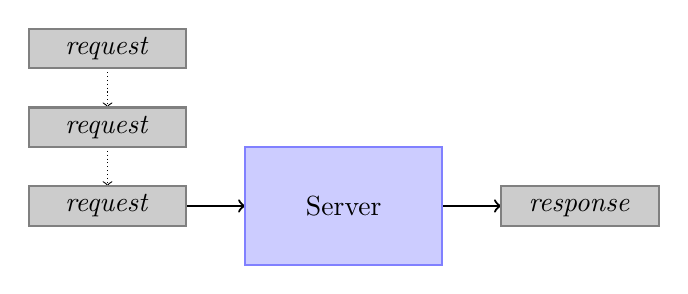
\begin{tikzpicture}[
          http/.style={fill=black!20,draw=black!50,thick},
          pending/.style={densely dotted,->},
        ]
        \draw[thick, ->] (-2, 0) -- (-1.25, 0);
        \draw[thick, ->] (1.25, 0) -- (2, 0);
        \draw[pending]   (-3, 1.75) -- (-3, 1.25);
        \draw[pending]   (-3, 0.75) -- (-3, 0.25);

        \draw[fill=blue!20,draw=blue!50,thick] (-1.25, -0.75) rectangle (1.25, 0.75);
        \draw[http] (-4, 1.75) rectangle (-2, 2.25);
        \draw[http] (-4, 0.75) rectangle (-2, 1.25);
        \draw[http] (-4, -0.25) rectangle (-2, 0.25);
        \draw[http] (2, -0.25) rectangle (4, 0.25);

        \path (0, 0) node {Server};
        \path (-3, 2) node {\emph{request}};
        \path (-3, 1) node {\emph{request}};
        \path (-3, 0) node {\emph{request}};
        \path (3cm, -1pt) node {\emph{response}};
      \end{tikzpicture}
    \end{center}
\end{enumerate}

\subsubsection{Boxes}
Flowcharts also have colored coded boxes. Each color has a meaning, they are as follows
\begin{enumerate}
  \item[\tikz{\draw[fill=blue!20,draw=blue!50,thick] (0,0) rectangle (9pt, 9pt);}] Blue boxes indicate functional components, ussually executeable code.
  \item[\tikz{\draw[fill=black!20,draw=black!50,thick] (0,0) rectangle (9pt, 9pt);}] Black boxes indicate data and static components. They are frequently used to represent data structures.
%  \item[\tikz{\draw (-9pt, -9pt) [fill=green!20,draw=green!50,thick] rectangle (-3pt, -3pt); \draw (3pt, -9pt) [fill=red!20,draw=red!50,thick] rectangle (9pt, -3pt);\draw[fill=yellow!35,draw=yellow!85,thick] (-4.5pt, 3pt) rectangle (4.5pt, 9pt);}]
  \item[\tikz{\draw[fill=green!20,draw=green!50,thick](0, 0) rectangle (9pt, 9pt);} \tikz{\draw[fill=yellow!35,draw=yellow!85,thick](0, 0) rectangle (9pt, 9pt);} \tikz{\draw[fill=red!20,draw=red!50,thick](0, 0) rectangle (9pt, 9pt);}]Green, Yellow and Red boxes ussually label states. They have no concrete meaning, but the stoplight color scheme is often used to show how components relate to one another.
\end{enumerate}

Figure~\ref{fig:agent-dispatch-flow} makes use of all of the principles discussed in this section, and so makes a good practical example.

\pagebreak

\section{Overview}

\subsection{The Main Modules}
The two main modules of Ekans are known as \emph{dispatch} and the \emph{agent pool}. Dispatch is responsible for establishing connections with new clients and handing them off to agents. The agents handle individual clients one at a time, serving their requests and dealing with errors.

Figure~\ref{fig:agent-dispatch-flow} 

\begin{figure}[H]
  \begin{center}
    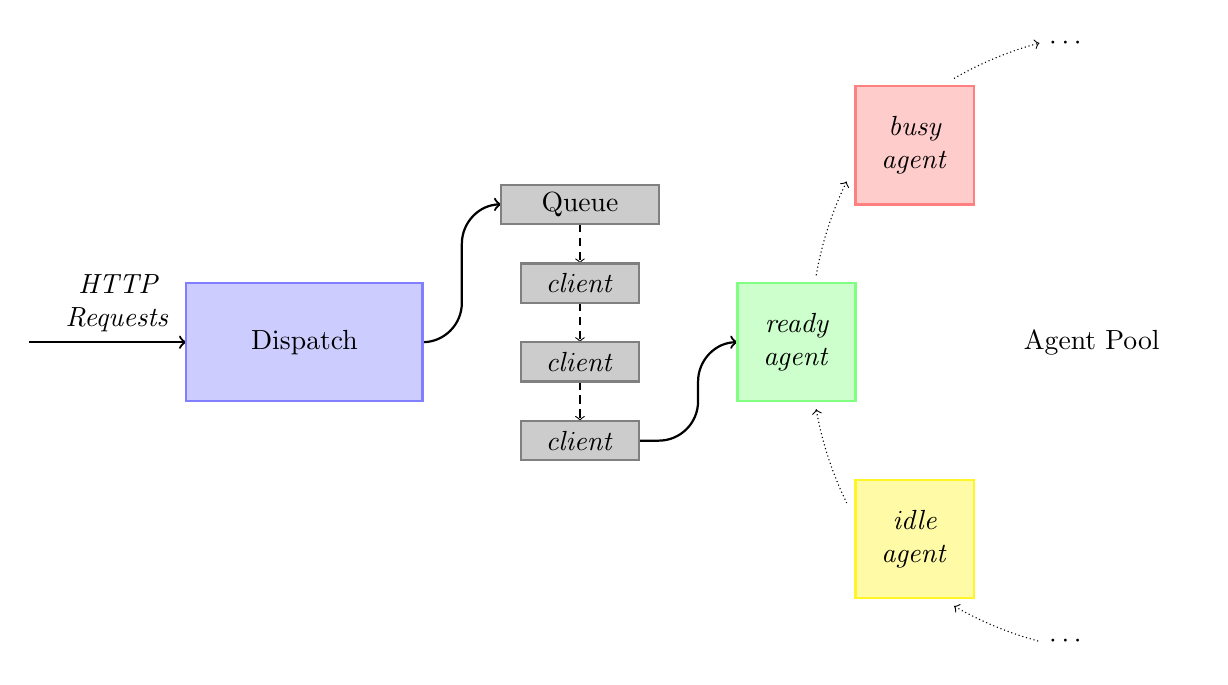
\begin{tikzpicture}[
        thick,
        queue/.style={fill=black!20,draw=black!50,thick},
      ]

      \draw[->,thick] (-5, 0) node[above right, text width=2cm, text centered] {\emph{HTTP Requests}} -- (-3, 0);
      \draw[densely dashed,->,thin] (2, 1.5) -- (2, 1);
      \draw[densely dashed,->,thin] (2, 0.5) -- (2, 0);
      \draw[densely dashed,->,thin] (2, -0.5) -- (2, -1);
      \draw[->,thick] (0, 0) arc (-90:0:0.5cm) -- (0.5,1.25) arc (180:90:5mm);
      \draw[->,thick] (2.75,-1.25) -- ++(0.25,0) arc (-90:0:5mm) -- ++(0, 0.25) arc (180:90:5mm);
      \draw[densely dotted,thin,->] (5, 0.85) arc (170:154:45mm);
      \draw[densely dotted,thin,->] (6.75, 3.35) arc (120:105:45mm) node[right] {$\cdots$};
      \draw[densely dotted,thin,<-] (5, -0.85) arc (190:206:45mm);
      \draw[densely dotted,thin,<-] (6.75, -3.35) arc (240:255:45mm) node[right] {$\cdots$};

      \draw[draw=blue!50,fill=blue!20,thick] (-3,-0.75) rectangle (0,0.75);
      \draw[queue] (1, 2) rectangle (3, 1.5);
      \draw[queue] (1.25, 1) rectangle (2.75, 0.5);
      \draw[queue] (1.25, 0) rectangle (2.75, -0.5);
      \draw[queue] (1.25, -1) rectangle (2.75, -1.5);
      \draw[draw=red!50,fill=red!20,thick] (5.5, 1.75) rectangle (7, 3.25);
      \draw[draw=green!50,fill=green!20,thick] (4, 0.75) rectangle (5.5, -0.75);
      \draw[draw=yellow!85,fill=yellow!35,thick] (5.5, -1.75) rectangle (7, -3.25);

      \path (-1.5, 0) node {Dispatch};

      \path (2, 1.75) node {Queue};
      \path (2, 0.75) node {\emph{client}};
      \path (2,-0.25) node {\emph{client}};
      \path (2,-1.25) node {\emph{client}};
      \path (6.25, 2.5) node[text centered,text width=1.5cm] {\emph{busy agent}};
      \path (6.25, -2.5) node[text centered,text width=1.5cm] {\emph{idle agent}};
      \path (4.75, 0) node[text centered,text width=1.5cm] {\emph{ready agent}};
      \path (8.5, 0) node[text centered,text width=2.5cm] {Agent Pool};

    \end{tikzpicture}
  \end{center}\caption{High level interactions of dispatch and the agent pool.}\label{fig:agent-dispatch-flow}
\end{figure}



\end{document}
